
 
\documentclass{beamer} 
\usepackage[utf8]{inputenc}
\usepackage{graphicx}
\usepackage{float}
\usepackage{multicol}
\usepackage{wrapfig}
\usepackage{multirow}
\usepackage{subcaption}
\usepackage{wrapfig}
\graphicspath{ {../report/images/} }
%\usetheme{Madrid}
\usecolortheme{beaver} 
\setbeamertemplate{footline}[frame number]


%Information to be included in the title page:
\title{Comparison of CORSIKA hadronic interaction models with GRAPES-3 experiment data}
\author{Mohit Saharan}
\institute{GRAPES-3 Interaction Meeting}
 
\begin{document}

\frame{\titlepage}


\begin{frame}{Outiline}
\begin{itemize}
    \item Introduction
    \item Cosmic Ray Induced air Showers
    \item GRAPES-3 experiment
    \item CORSIKA simulation program
    \item Comparison of different CORSIKA hadronic interaction generators with GRAPES-3 data
    \item Comparison of CORSIKA simulation data with GRAPES-3 data
    \item Summary
\end{itemize}
\end{frame}


\begin{frame}{Cosmic Rays}


\begin{wrapfigure}{R}{5cm}
%\centering
	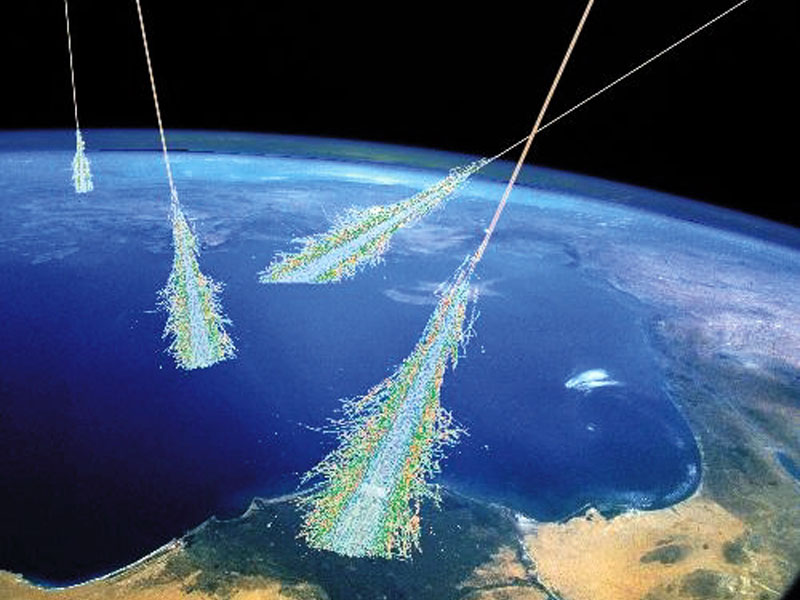
\includegraphics[width=0.9\linewidth, height=4.4cm]{cosmic_rays} 
\caption{Schematic of GRAPES-3 detector array}
\label{fig:cosmic_rays}
\end{wrapfigure}


\begin{itemize}
    \item One of the main challenges of astroparticle physics is to understand the source and propagation of cosmic rays.	
    \item What are Cosmic rays?
    \begin{itemize}
    	\item Charged particles from extra-terrestrial origin bombarding Earth’s atmosphere.
    	\item Energy varies from less than 1 GeV to $10^{20}$ eV.
    	\item Only indirect measurements possible for energies $\geq10^{14}$ eV (Extensive Air Showers)
    \end{itemize}
     	
\end{itemize}
\end{frame}


\end{document}